%Place here all the mockups
\subsection{Web Interface}
The following mockups show how the interface of the Web Application should look like on the user's browser.

\begin{figure}[H]
\centering
		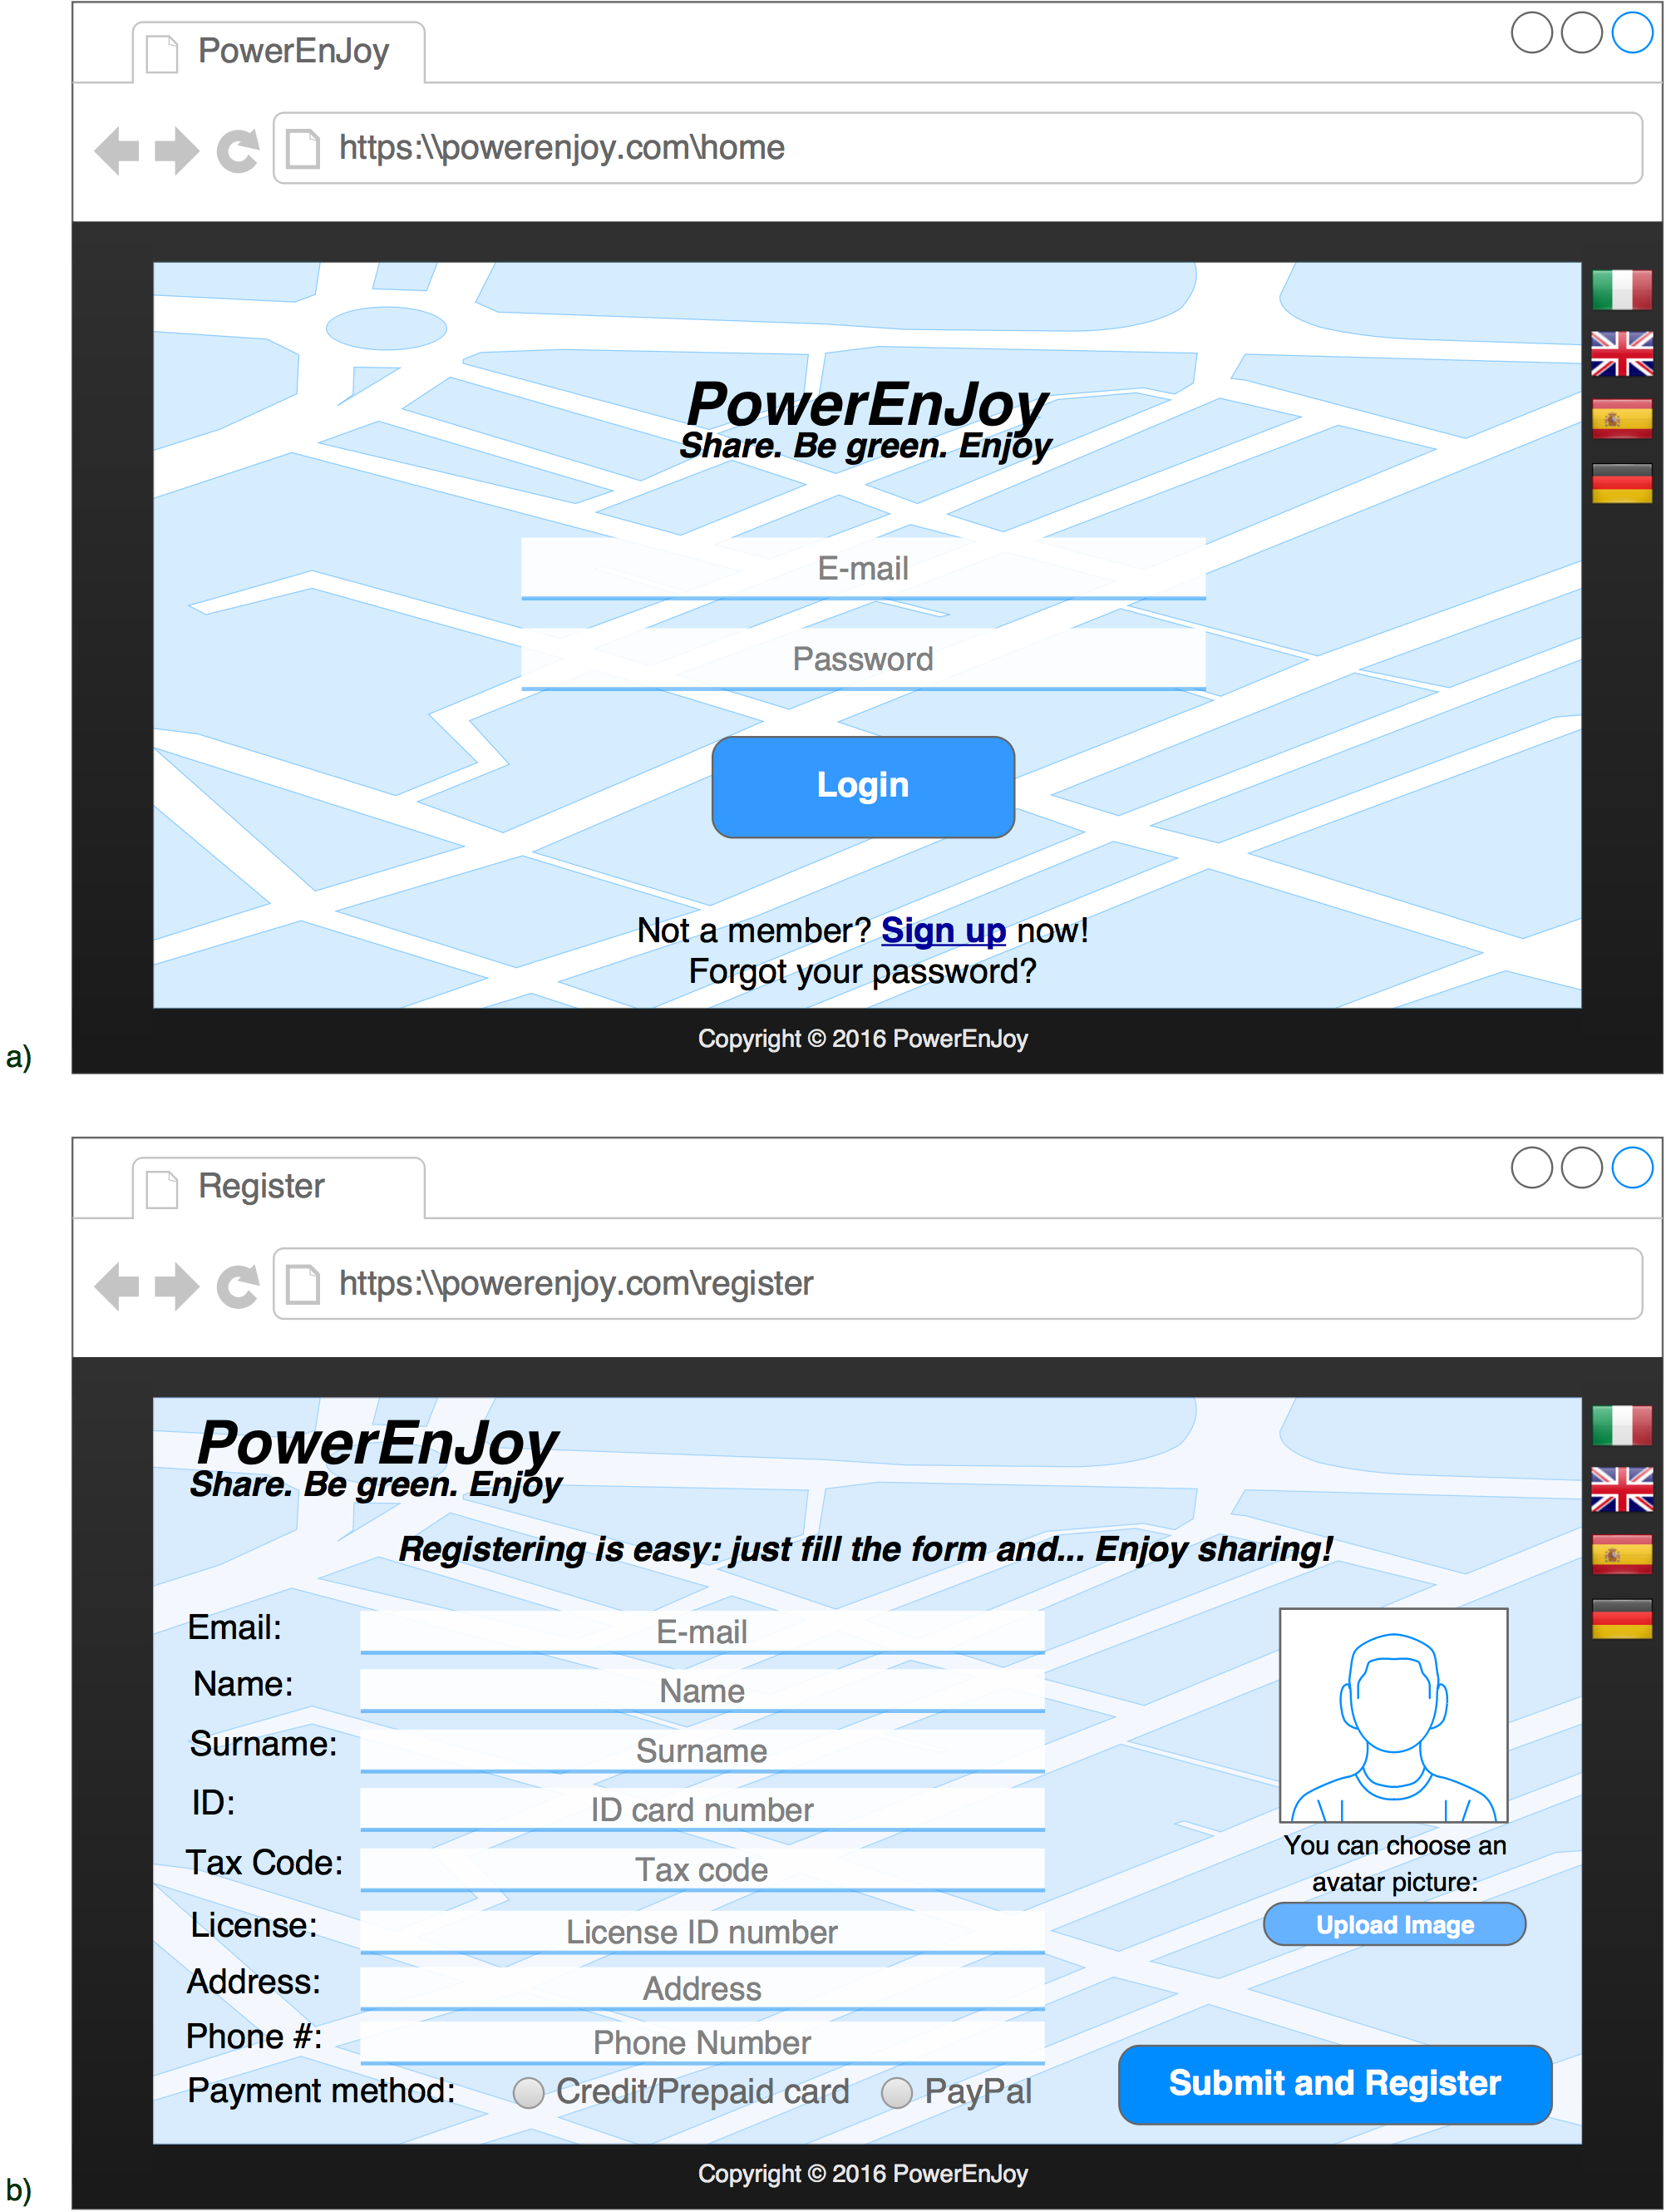
\includegraphics[width=\textwidth]{./user_interface_design/diagrams/web_login_register.png}
		\caption{Look and feel of the "Home" screen (a) and the "Registration" screen (b).}
		\label{web_login_register}
\end{figure}

\begin{figure}[H]
\centering
		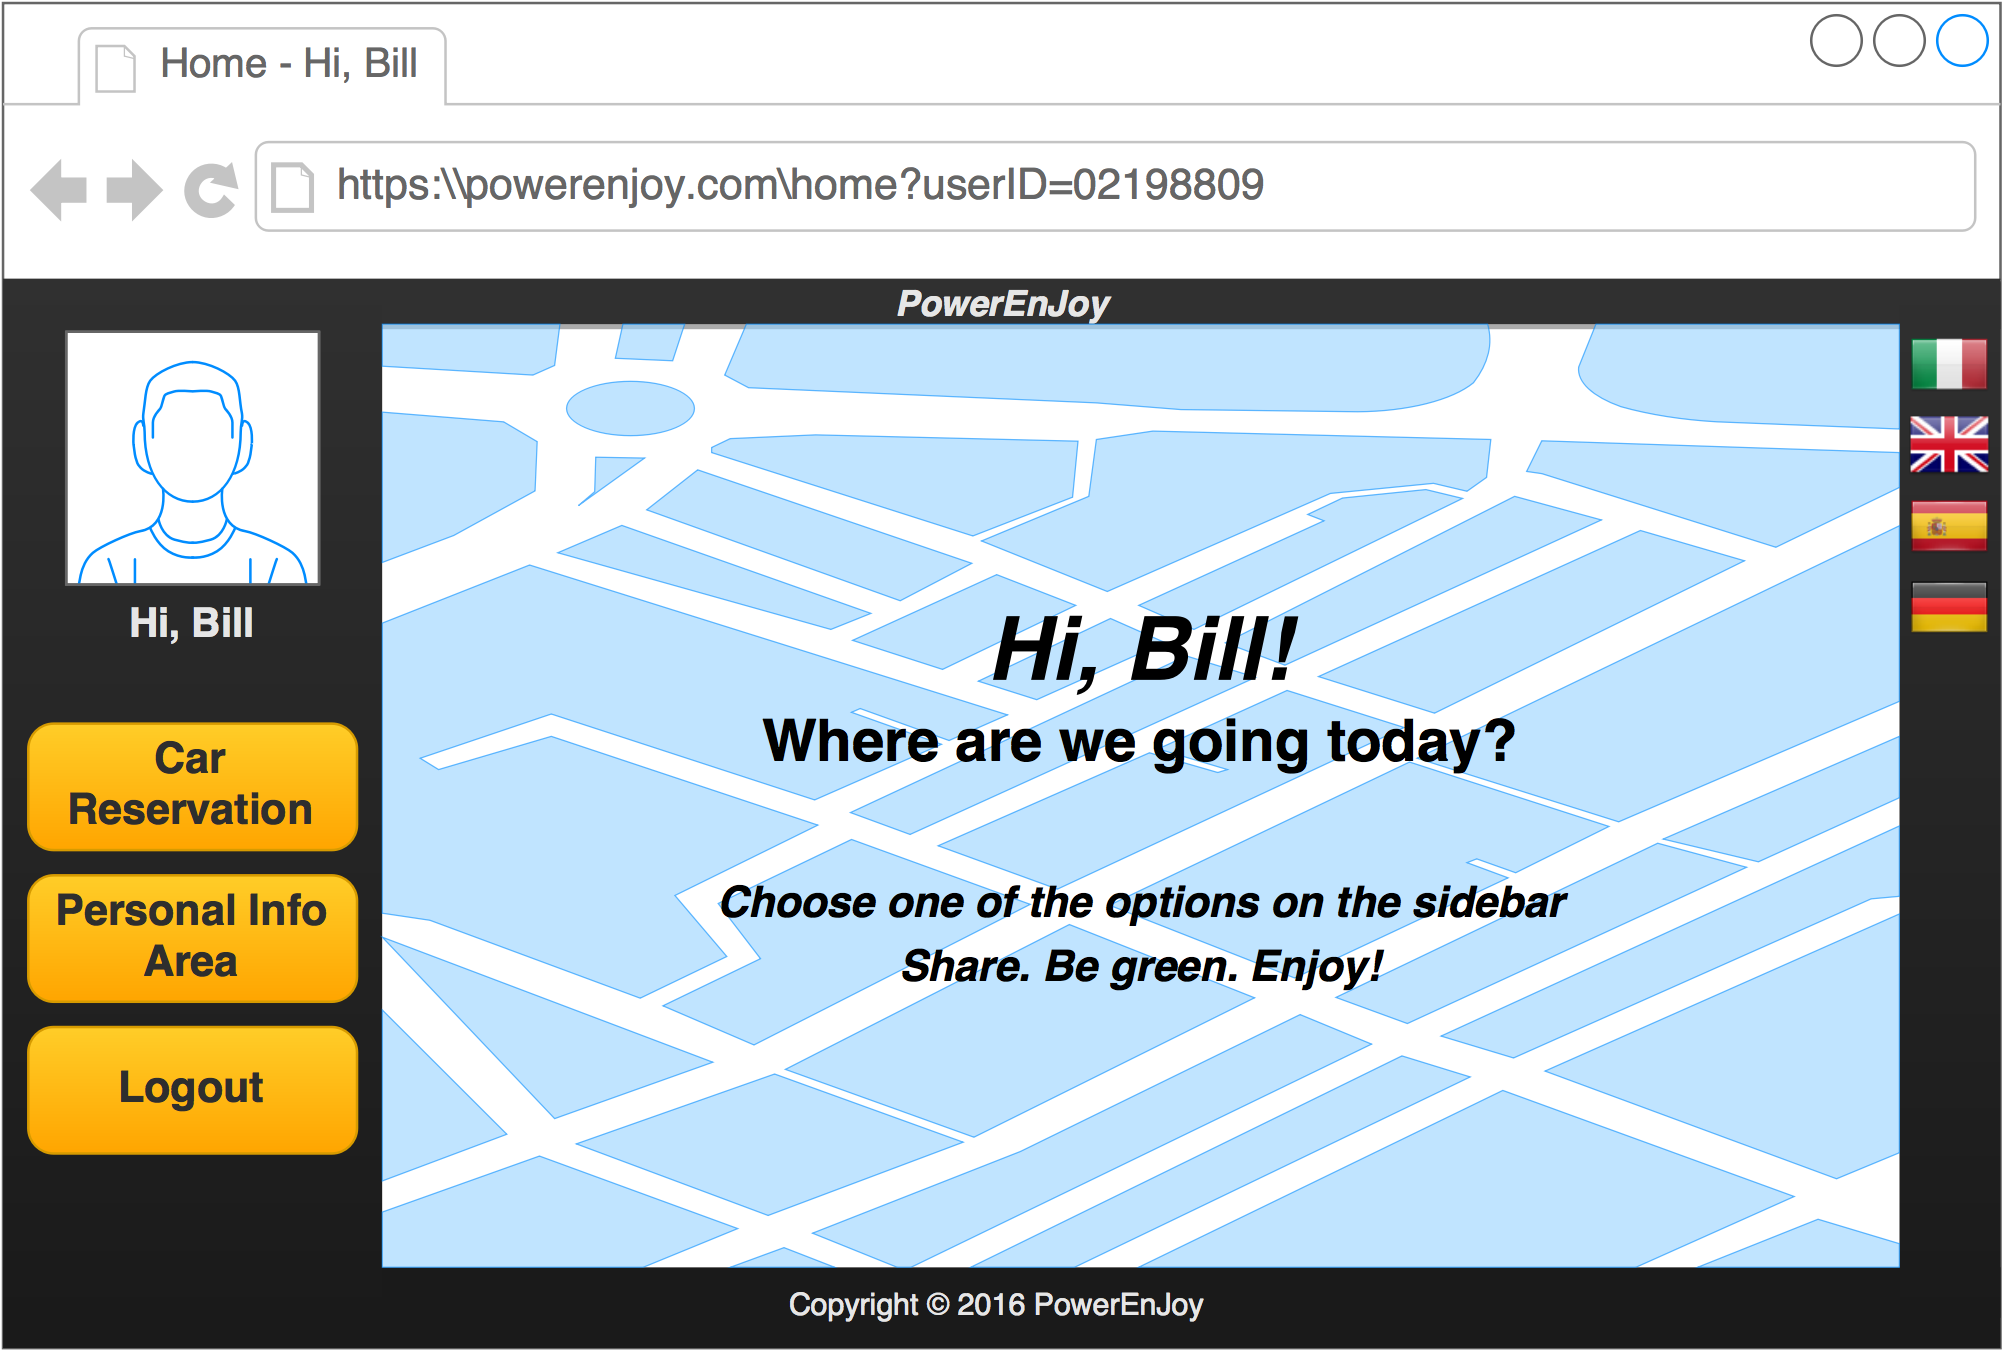
\includegraphics[width=\textwidth]{./user_interface_design/diagrams/web_user_home.png}
		\caption{Look and feel of the "User Home" screen.}
		\label{web_user_home}
\end{figure}

\begin{figure}[H]
\centering
		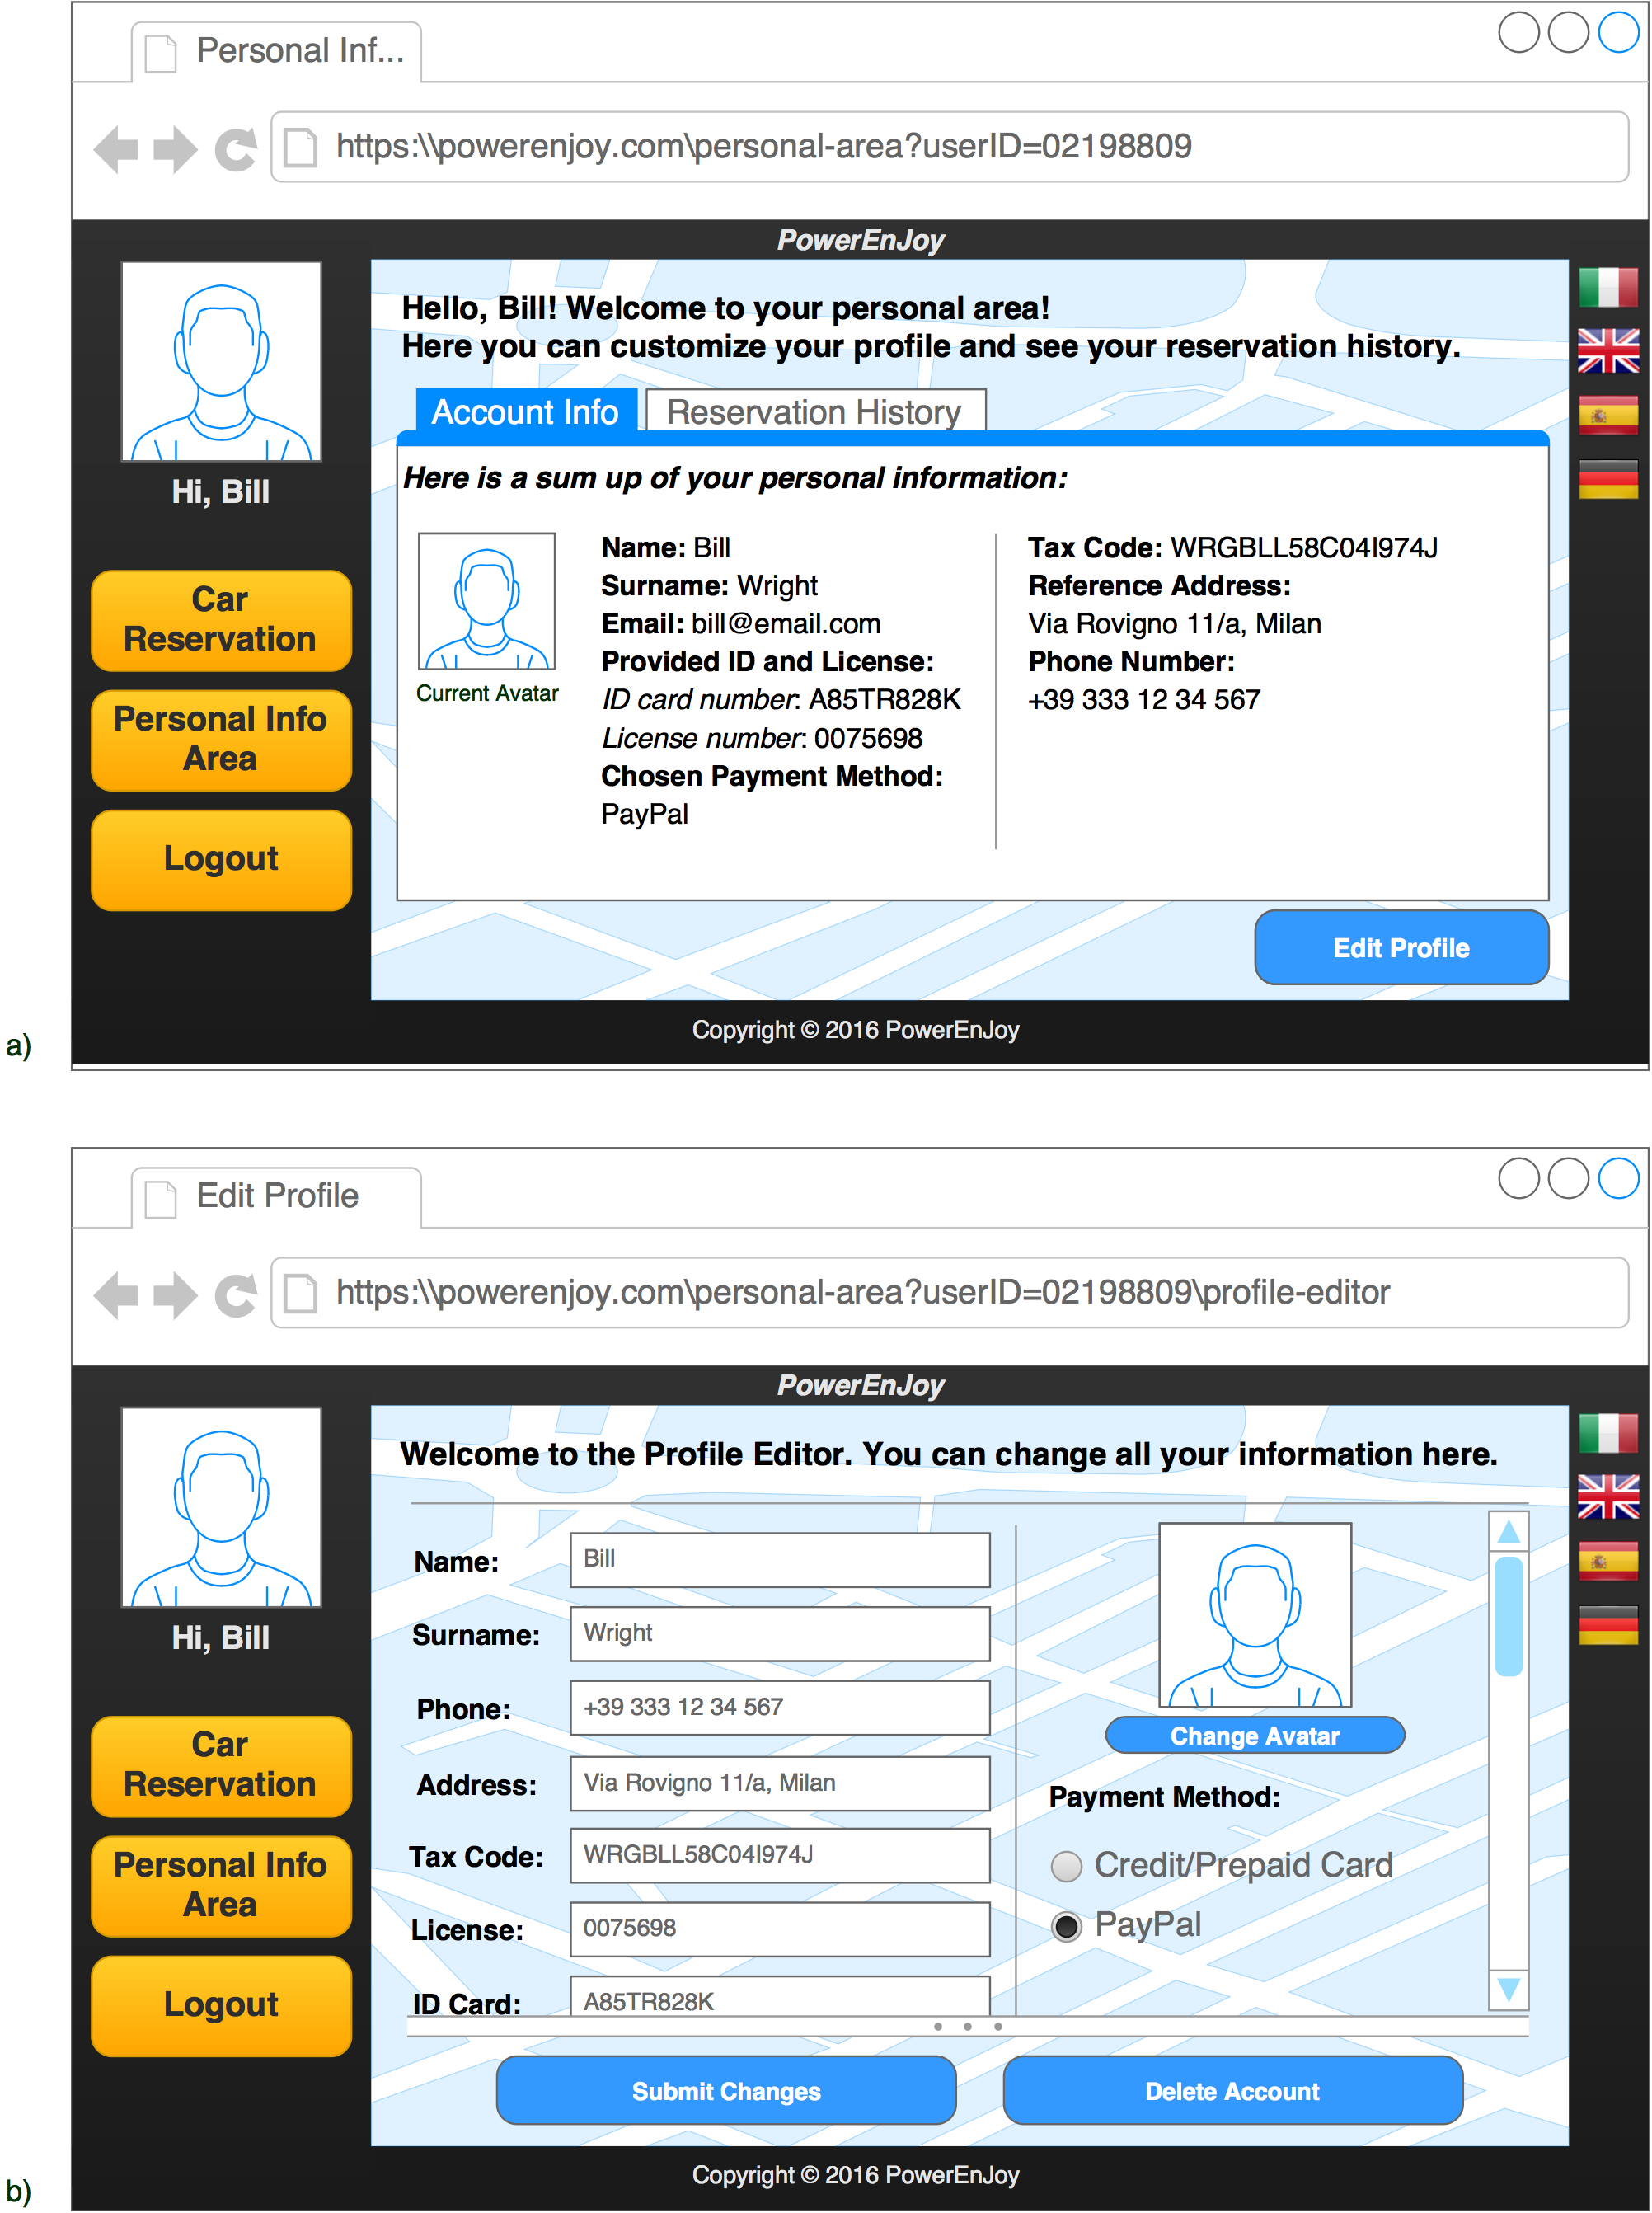
\includegraphics[width=\textwidth]{./user_interface_design/diagrams/web_personal_info_editor.png}
		\caption{Look and feel of the "Personal Information Area" screen (a) and the "Profile Editor" screen (b).}
		\label{web_personal_info_editor}
\end{figure}

\begin{figure}[H]
\centering
		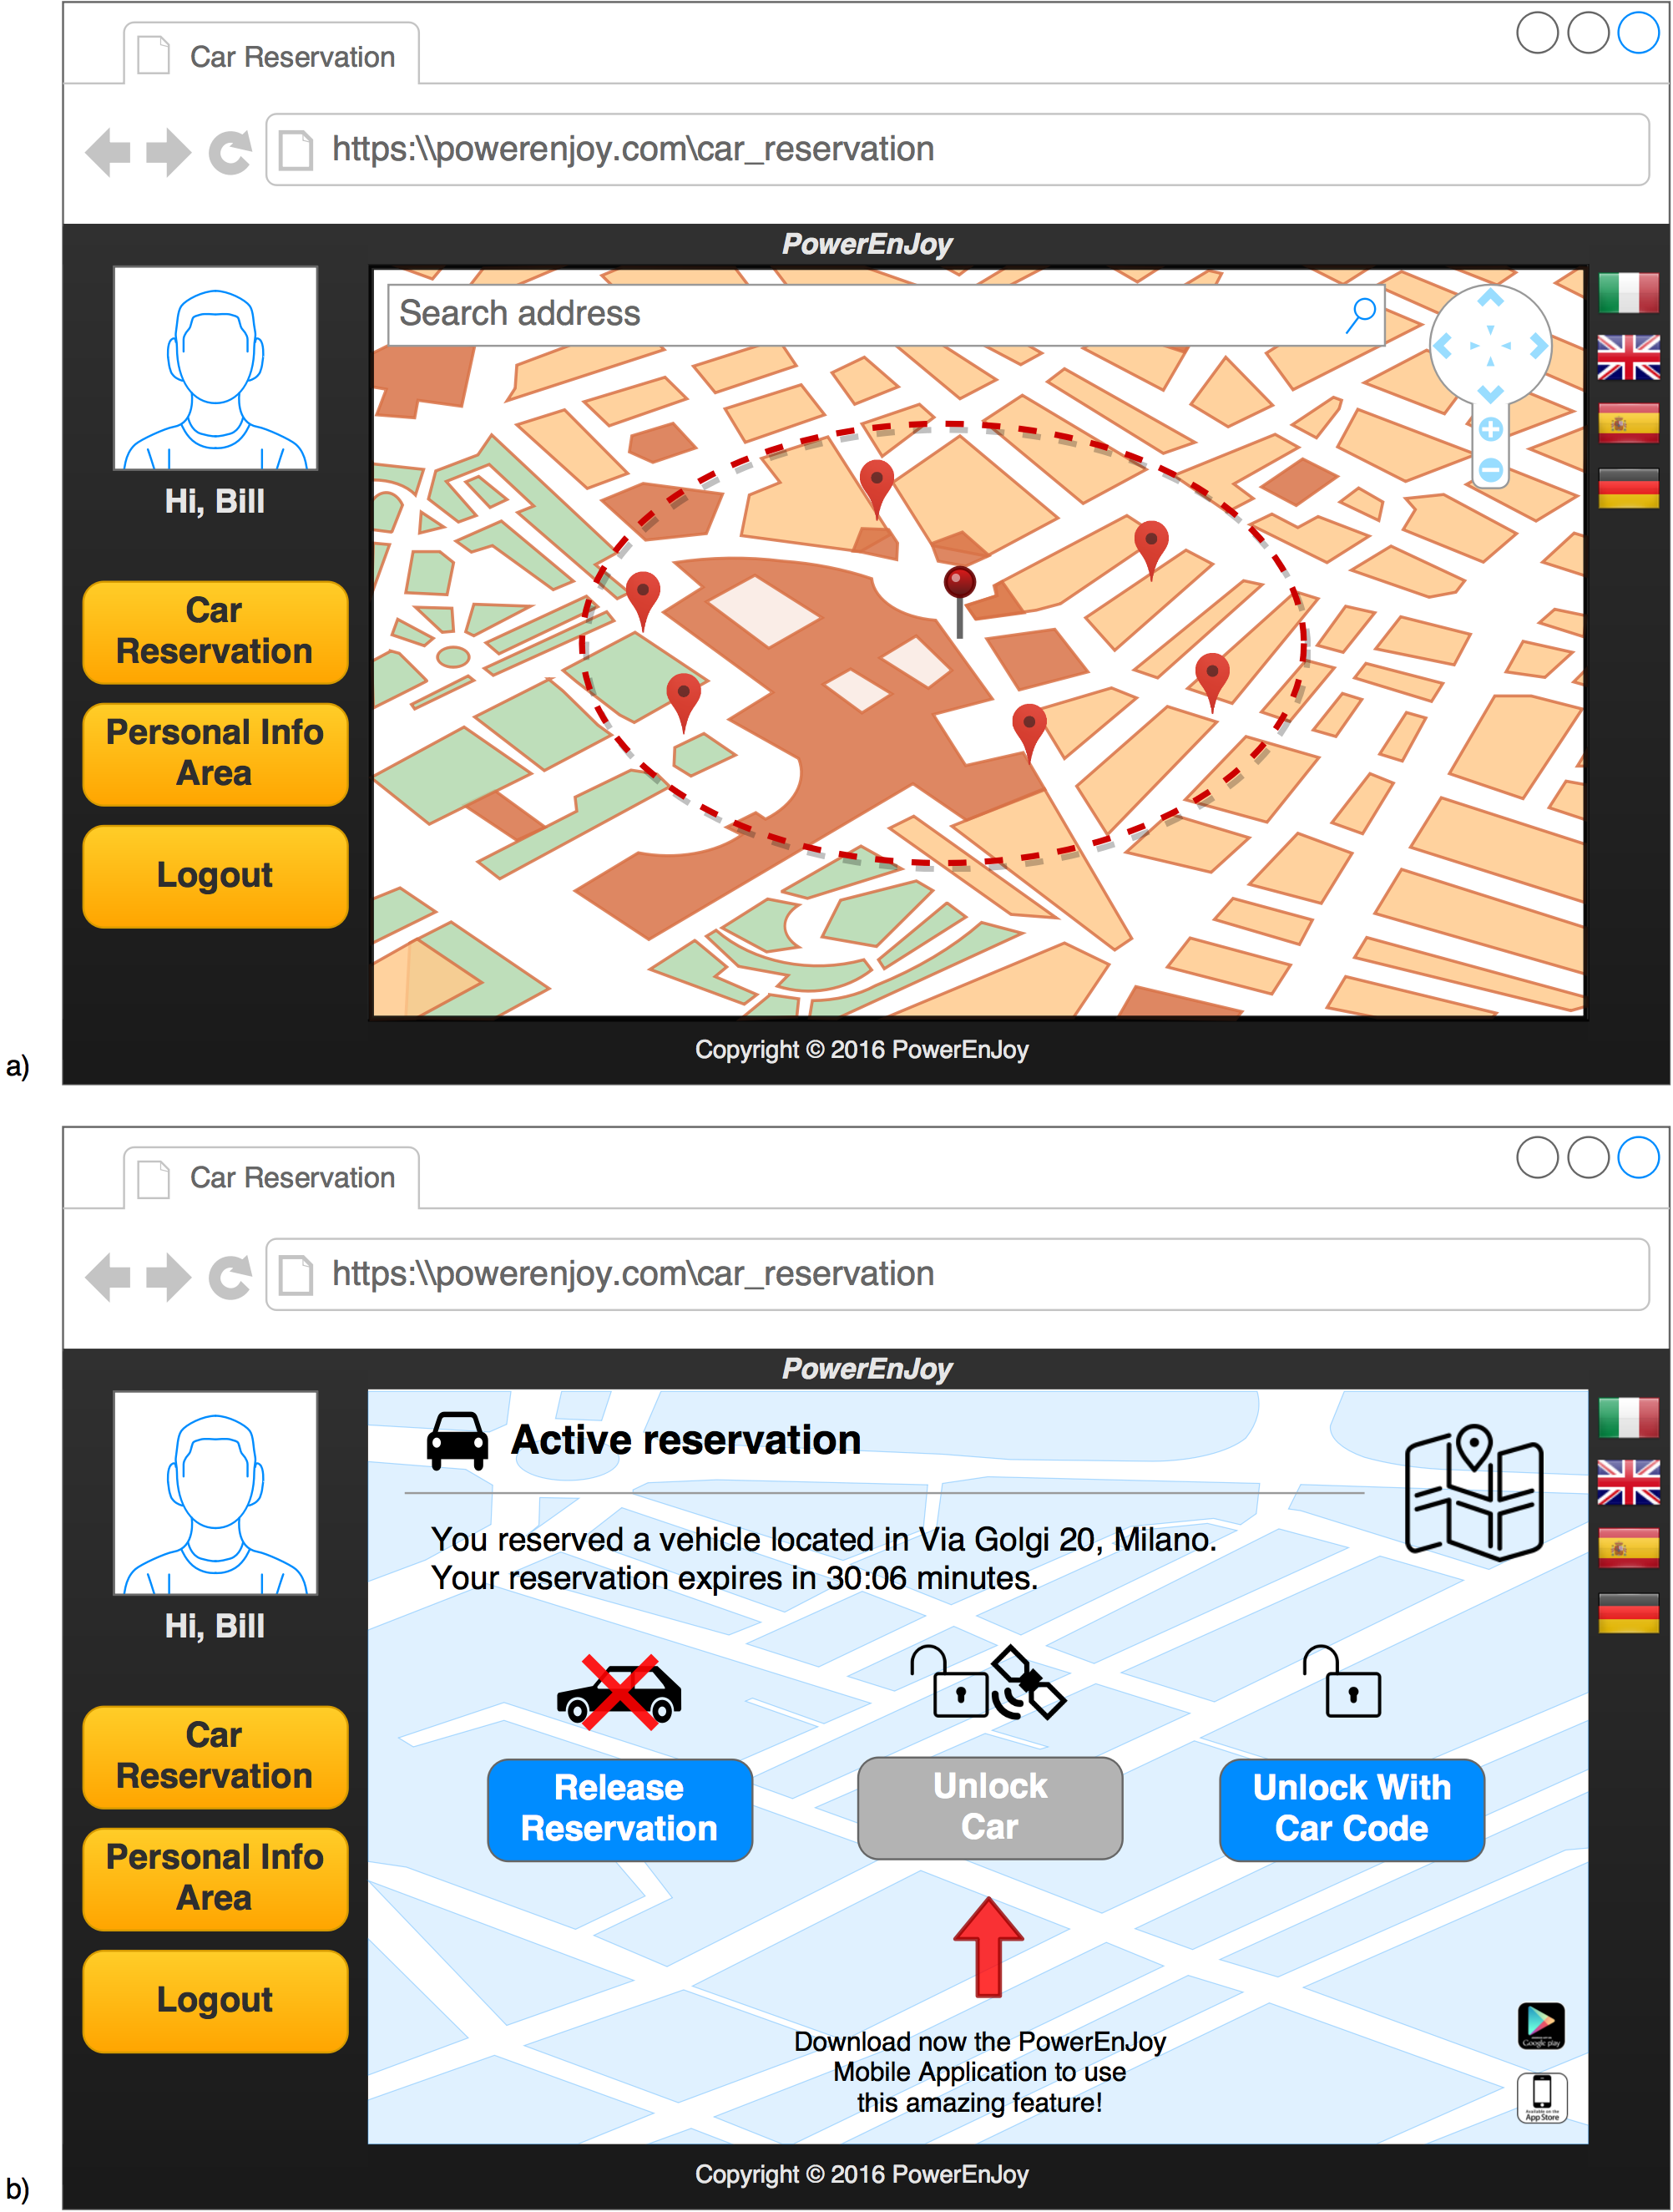
\includegraphics[width=\textwidth]{./user_interface_design/diagrams/web_car_reservation.png}
		\caption{Look and feel of the "Reserve A Car" screen (a) and the "Active Reservation" screen (b). They are both accessible from the "Car Reservation" button in the toolbar: the first is loaded if the user has no active reservation while the second otherwise.}
		\label{web_car_resrvation}
\end{figure}

\subsection{Mobile Interface}
The following mockups show how the interface of the Mobile Application should look like on the user's smartphone.

\begin{figure}[H]
\centering
		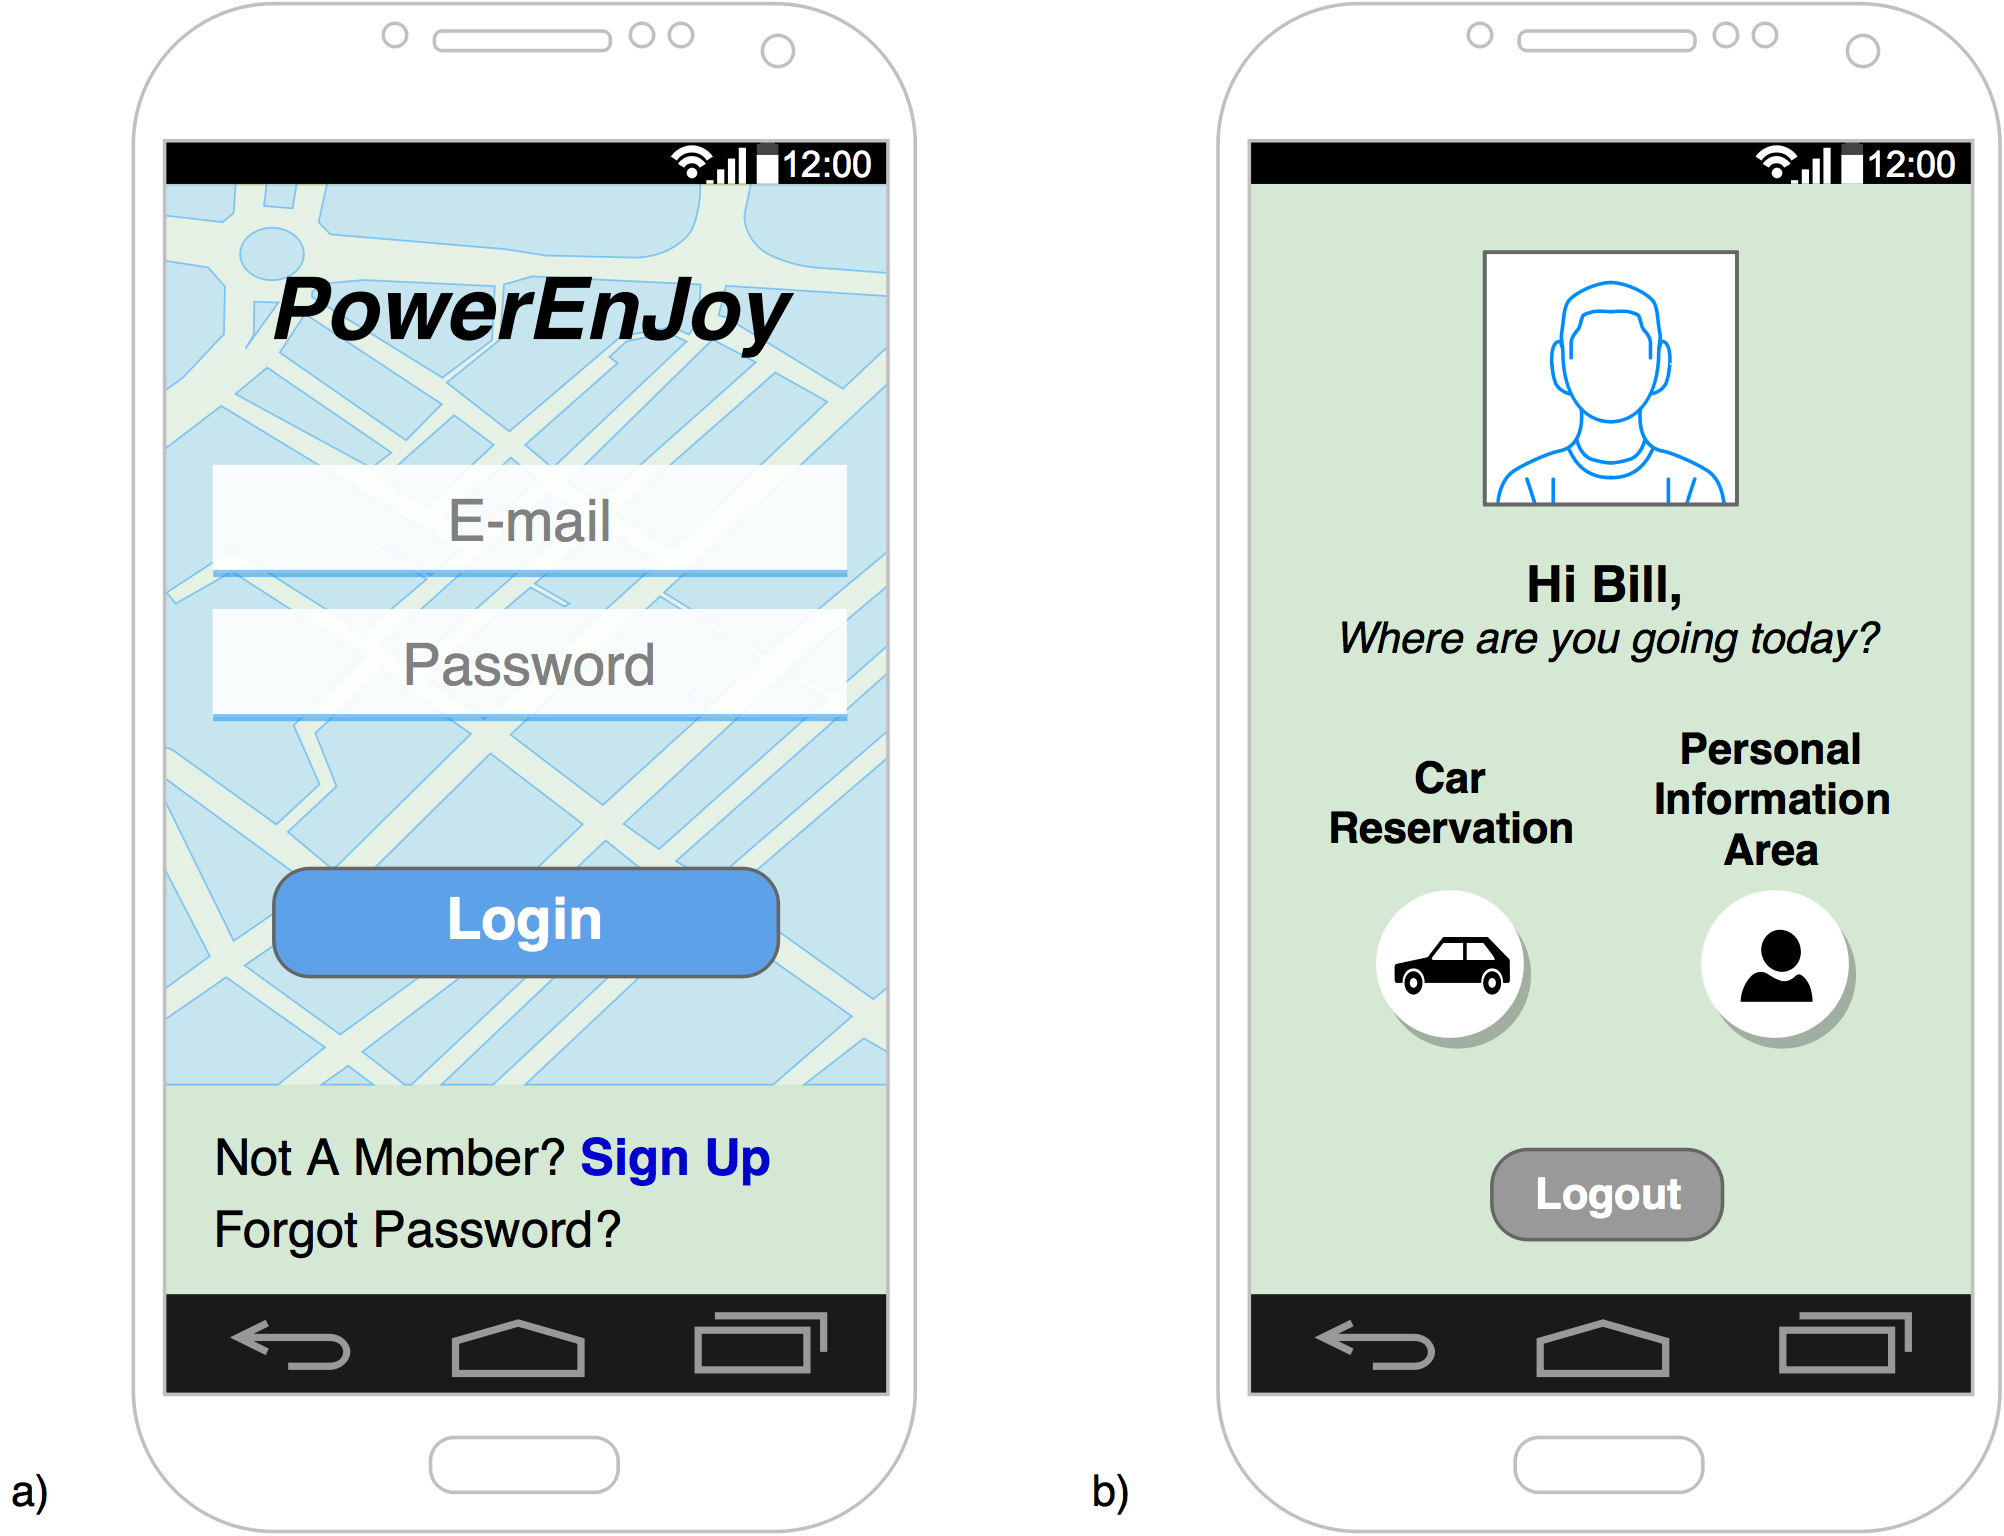
\includegraphics[width=\textwidth]{./user_interface_design/diagrams/mobile_login_home.png}
		\caption{The "Login" screen (a) and the "User Home" screen (b) of the Mobile Application.}
		\label{mobile_login_home}
\end{figure}

\begin{figure}[H]
\centering
		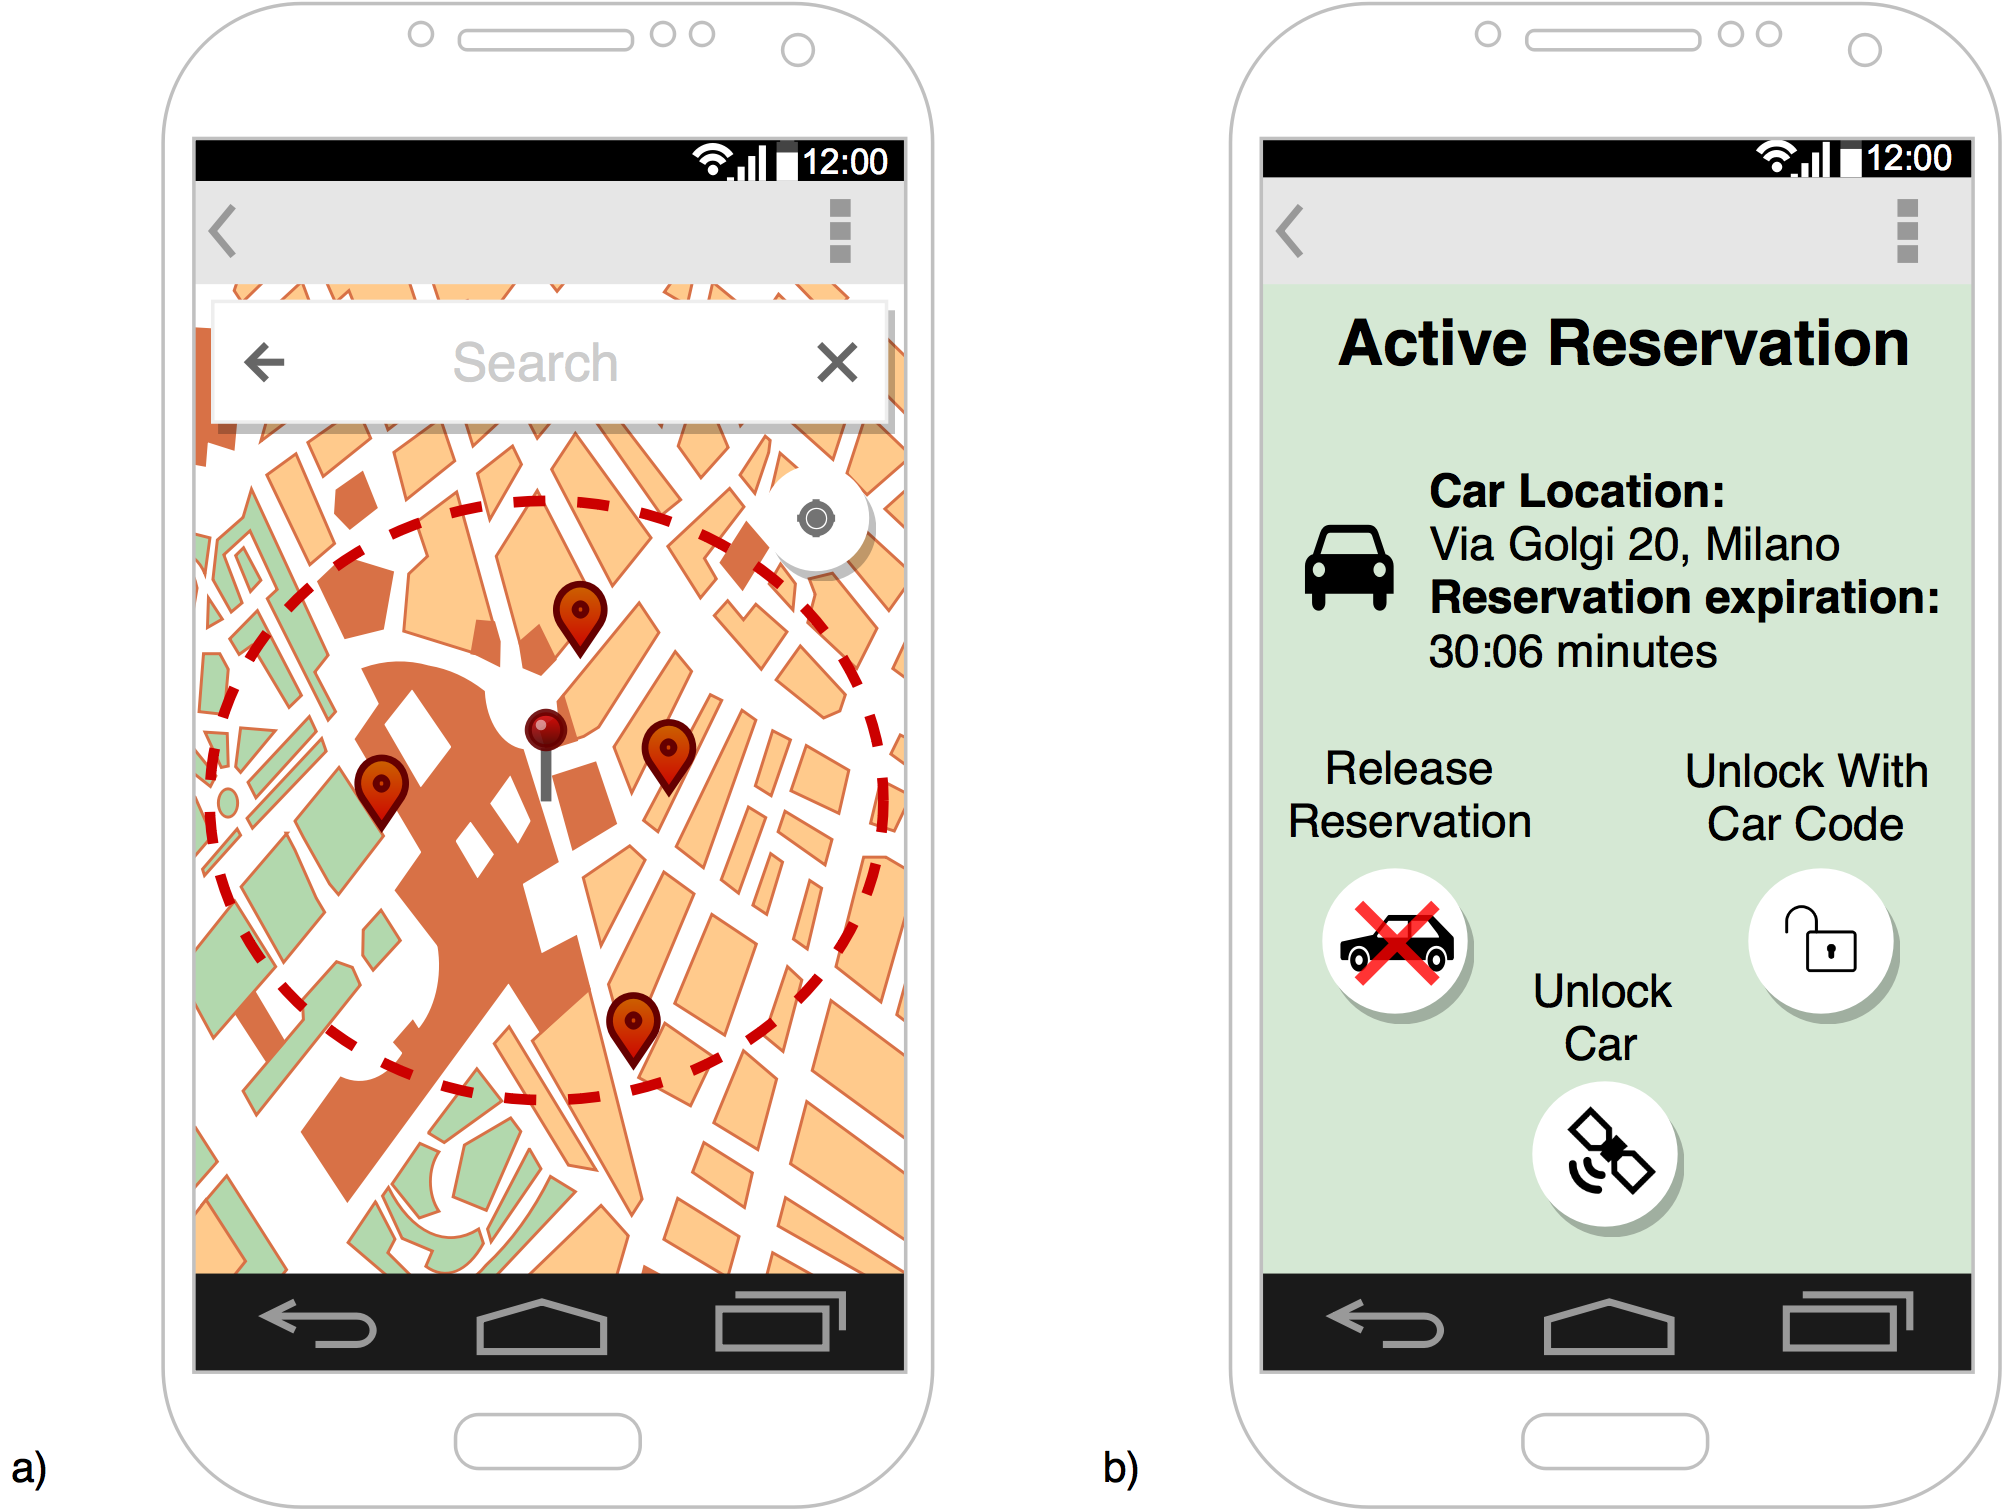
\includegraphics[width=\textwidth]{./user_interface_design/diagrams/mobile_res_unlock.png}
		\caption{Look and feel of the "Reserve A Car" screen (a) and the "Active Reservation" screen (b). They are both accessible from the "Car Reservation" button in the "User Home" screen: the first is loaded if the user has no active reservation while the second otherwise.}
		\label{mobile_res_unlock}
\end{figure}

\subsection{On-Board Interface}
The following mockups show how the interface of the On-Board Application should look like on the on-board computers of cars.

\begin{figure}[h]
\centering
		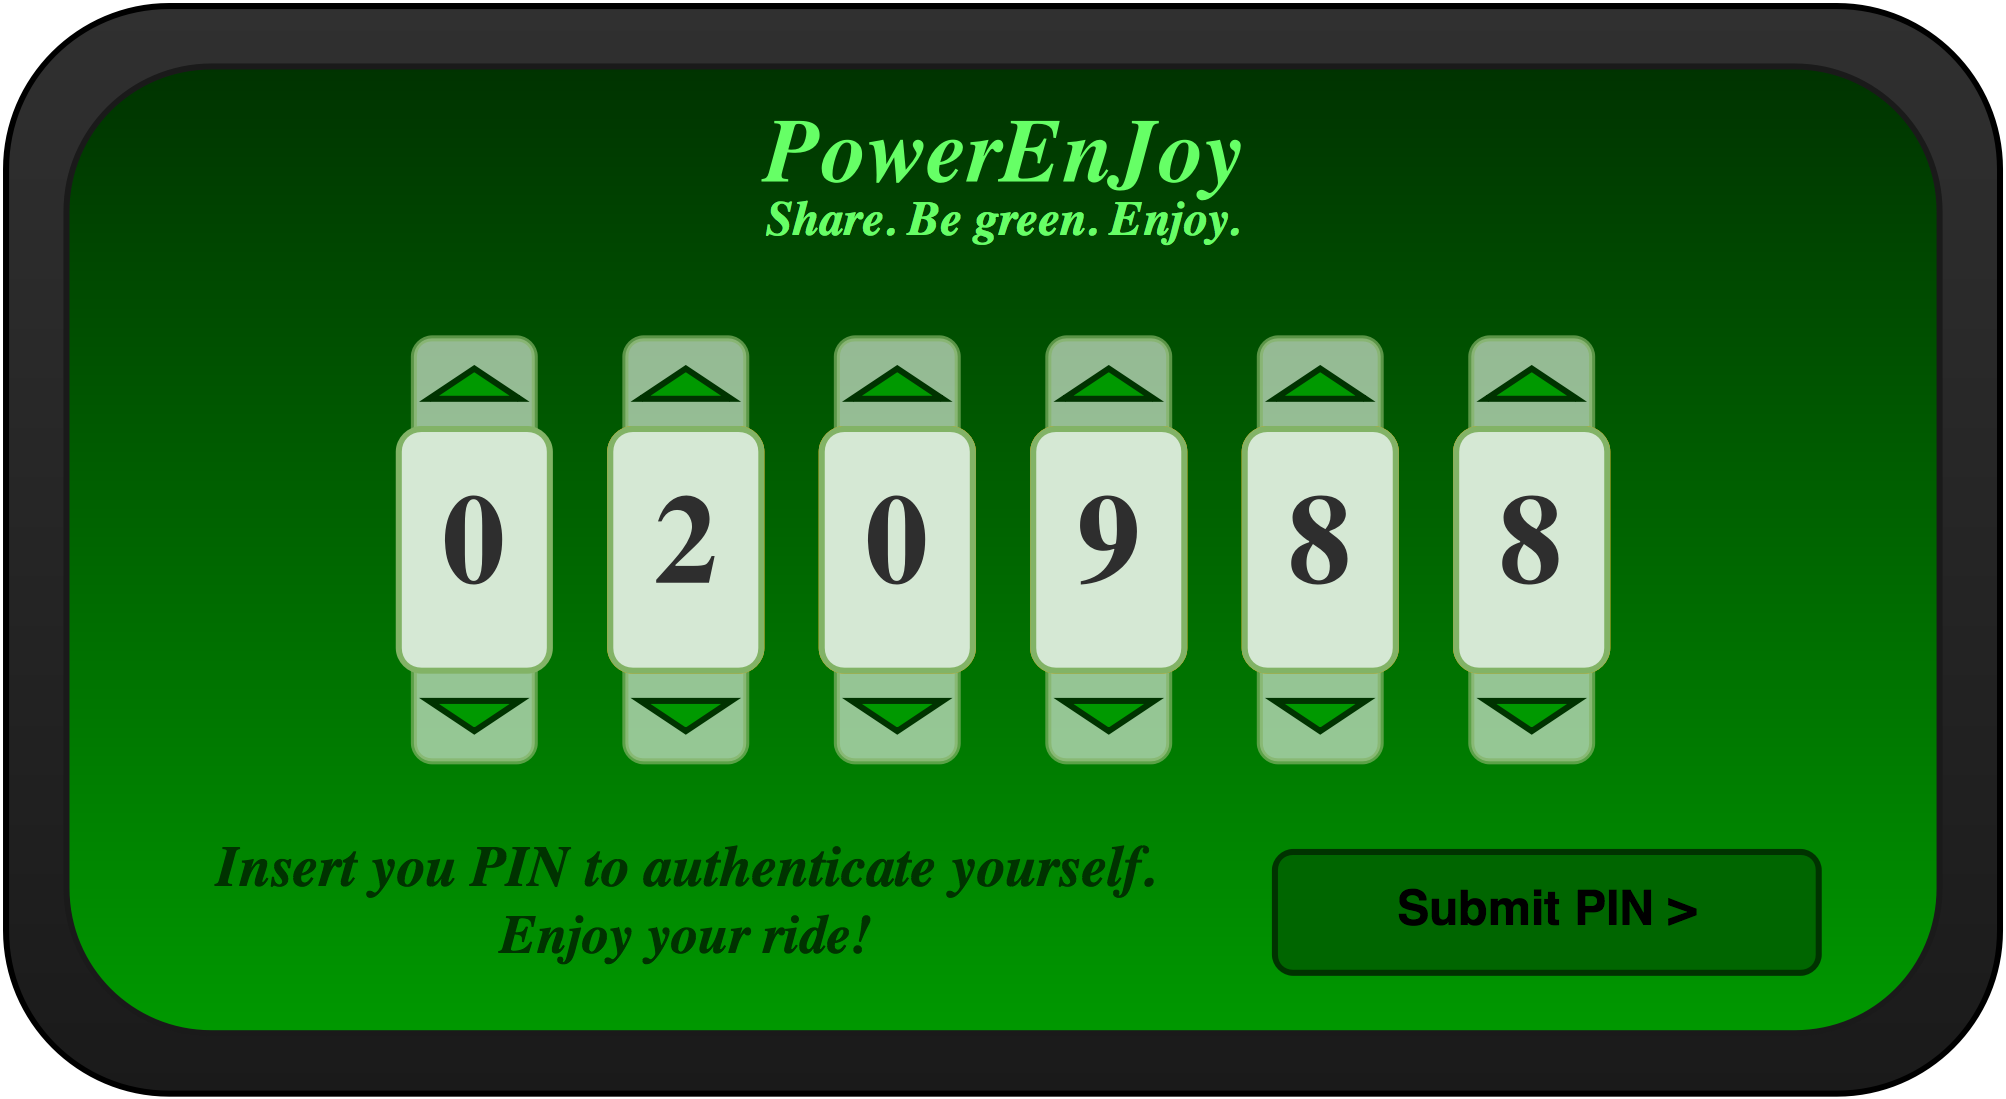
\includegraphics[width=\textwidth]{./user_interface_design/diagrams/onboard_auth.png}
		\caption{Concept of the looks of the "Authentication" screen on the on-board touch screen.}
		\label{onboard_auth}
\end{figure}

\begin{figure}[h]
\centering
		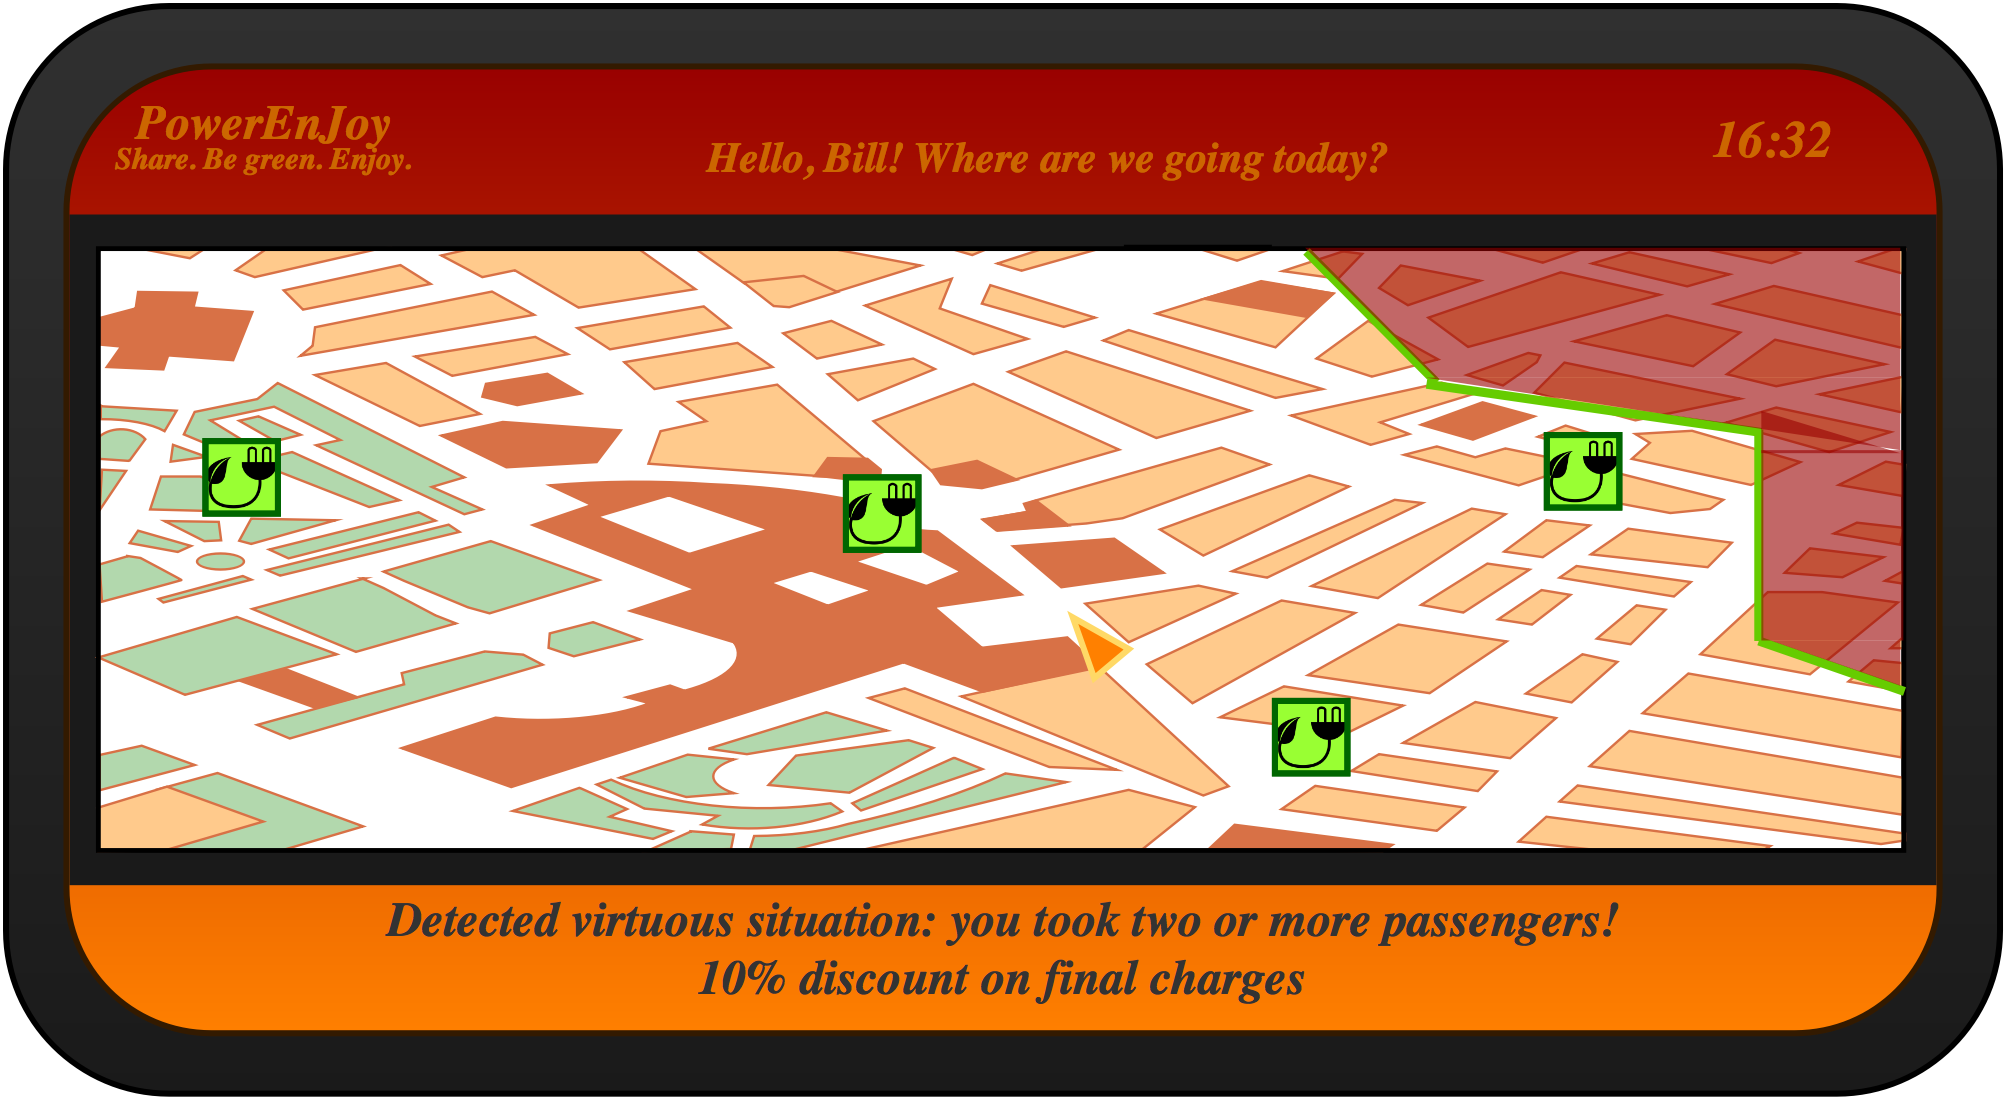
\includegraphics[width=\textwidth]{./user_interface_design/diagrams/onboard_ride.png}
		\caption{Concept of the looks of the "Ride Status" screen on the on-board touch screen.}
		\label{onboard_ride}
\end{figure}